%------------------------------------------------------------------------------
\begin{frame}
    \frametitle{Problem Definition}
    2D square plate of side 1 m with one hot side and other 3 cold sides
    \begin{figure}
        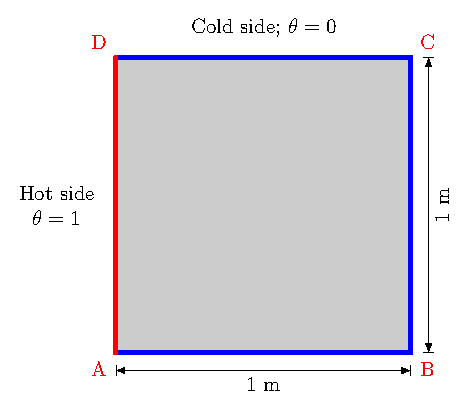
\includegraphics[scale=0.7]{00_schematic/01_problem_schematic/problemDefinition.pdf}
    \end{figure}

    Present work is to compute the temperature field within plate domain
    using PINNs with different variations in methodology.
\end{frame}

%------------------------------------------------------------------------------
\begin{frame}
    \frametitle{Governing equation and Analytical solution}

    \begin{figure}
        \centering
        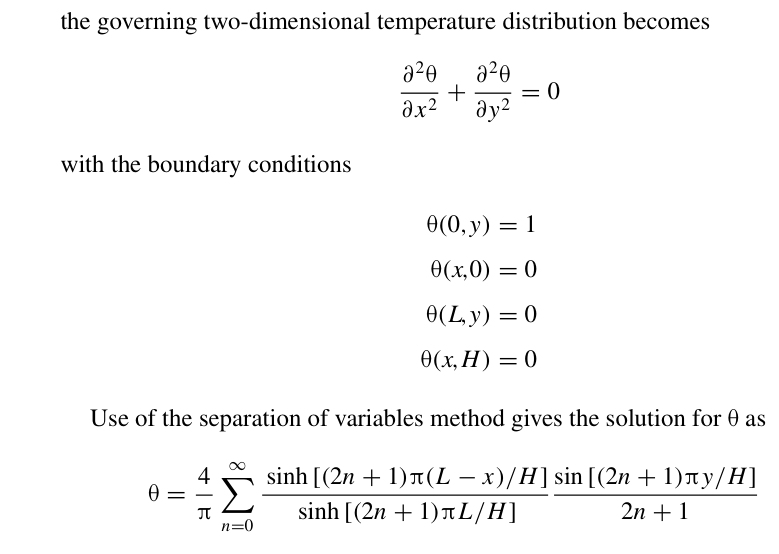
\includegraphics[scale=0.4]{supportingFiles/eqn.png}
    \end{figure}
\end{frame}

%------------------------------------------------------------------------------

\begin{frame}
    \frametitle{Network Schematic}
    \begin{figure}
        \centering
        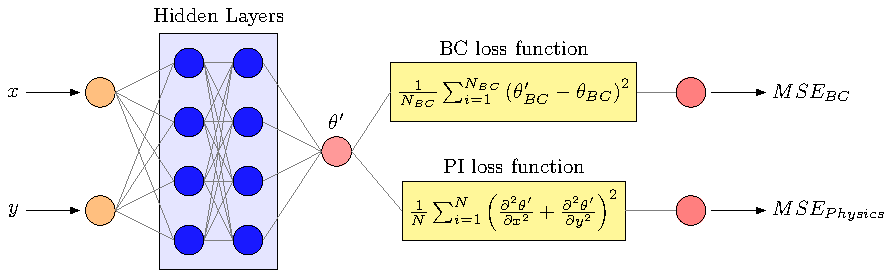
\includegraphics[scale=0.77]{00_schematic/02_PINN_schematic/PINN_HC_schematic.pdf}
    \end{figure}
\end{frame}
